\chapter{Implementation}
\label{chap:implementation}

In this chapter, it is described how the AI-based malaria classification system was implemented based on the concept developed in Chapter~\ref{chap:concept-development}. It explains the dataset used for the implementation, the preprocessing pipeline, the software tools (such as PyTorch, torchvision and Matplotlib), and the structure of the developed pipeline.
This chapter also explains how the individual components (dataset loading, preprocessing, training, testing and Grad-CAM Analysis) are connected and how reproducibility is supported through fixed data splits, saved model checkpoints, and version-controlled development.

\section{Data Acquisition}

The image data used for the implementation was obtained from publicly available malaria microscopy datasets. No new blood smear images were collected as part of this thesis. 

The training, validation, and main evaluation were based on the NLM/NIH thick blood smear dataset, which has also been used by Kassim et al. \cite{Kassim2021}. It was decided that the NLM/NIH dataset was the perfect match for the developed model because it contains thick blood smear images from infected and uninfected patients, which means it fits the binary classification task of this thesis. Another important advantage is its patient-based structure, which makes it easy to separate the data at patient level and avoid images from the same patient appearing in both training and evaluation sets.

Two additional public datasets were considered during the dataset selection. The Uganda microscopy dataset described by Quinn et al. \cite{Quinn2016} contains thick blood smear images with parasite annotations and is more suitable for parasite detection and localisation tasks. This dataset is available for download on the official website of AIR Uganda which belongs to Makerere University. The Uganda dataset was later used only for an external test of the trained models to check whether the predictions depend strongly on dataset-specific image characteristics. The second dataset is the Vall d'Hebron dataset \cite{VallHebron2025} which also contains labelled thick blood smear images, but mainly provides malaria-positive samples. This one is also not suitable for the infected-versus-uninfected classification used in this work. To get access to this dataset, an application was submitted, and access to the dataset was granted afterwards. 

The Vall d'Hebron dataset was obtained as a possible data source for a future extension of the project, for example towards parasite detection or species identification.

No image data from the Ethiopian Artificial Intelligence Institute were available for the implementation of this thesis. The developed AI method and the other components of the overall project are intended to be transferred to EAII for later development and testing.

\section{Dataset Description}
\label{sec:dataset-description}

As explained in the previous section, the NLM dataset is the most suitable dataset for this work. It consists of three thick blood smear subsets which contain images from uninfected patients, patients infected with Plasmodium vivax, and patients infected with Plasmodium falciparum. All these three subsets contain Giemsa-stained thick blood smear images acquired through the eyepiece of a microscope at 100$\times$ magnification using a smartphone camera. The original images are RGB images with a resolution of 3024 $\times$ 4032 pixels \cite{Yang2020,Kassim2021}.

The uninfected subset contains 1141 images from 50 malaria-negative patients \cite{Kassim2021}. The images are stored in TIFF format and are organised in separate folders by patient. The dataset also provides annotations for white blood cells, which are not needed for the whole-image classification used in this thesis.

 The P. vivax subset contains images from 150 malaria-infected patients, with approximately 20 images per patient \cite{Kassim2021}. Kassim et al. report in their paper a total of 3013 images, while 3014 images were found in the downloaded dataset and used in the implementation. The images are stored in JPEG format and parasite locations are provided in separate annotation files. Since the goal of this thesis is to classify complete images rather than identify individual parasites, these parasite annotations were also not used for the classification process.

The P. falciparum subset contains images from 150 infected patients, with approximately 12 images per patient \cite{Yang2020}. Yang et al. report a total of 1819 images, while 1883 images were found in the downloaded dataset and used in the implementation. These images are also stored in JPEG format. The corresponding annotation files contain information about parasite and white blood cell positions. Just like the P. vivax subset, these annotations were not required for the whole-image classification task.

For the classification task, the two infected subsets were combined into one positive class. Images from patients infected with P. vivax or P. falciparum were assigned to the class infected, while the images from the uninfected subset were assigned to the class uninfected. In total, 6038 images were included in the implementation: 1141 uninfected images, 3014 P. vivax images, and 1883 P. falciparum images. The final classification task therefore contains two output classes: infected and uninfected.

In addition to the NLM dataset, the Uganda microscopy dataset was used as an external test dataset \cite{Quinn2016}. It contains 1182 malaria-positive images stored in JPEG format. The dataset does not provide patient IDs, and all images used for this external evaluation were assigned to the test split. The Uganda dataset was kept completely separate from the training and validation process and is therefore not included in the 6038 NLM images described above.

\section{Data Preprocessing Pipeline}
\label{sec:data-preprocessing}

Before diving into training the model, the raw data must first be prepared in a way that makes it readable and consistent. This section walks through the preprocessing steps used in this work.

The preprocessing pipeline was implemented in the following steps: First, the image information and binary labels were prepared using the script \textbf{build\_labels.py}. The images were then loaded using the \textbf{MalariaDataset} class from the \textbf{dataset.py} script. After that, the required preprocessing transforms were applied for training, validation, and testing. These transforms are different depending on the split. Training images received random augmentation, while validation and test images did not. For the low-resolution experiments, the same images were reduced to the selected resolution before being resized back to \(224 \times 224\) pixels, which is the required input resolution for the model.

The script \textbf{build\_labels.py} goes through all three NLM image folders for \textbf{Uninfected}, \textbf{P. vivax}, and \textbf{P. falciparum} images. The binary labels are assigned based on the images folder. Images from the uninfected subset receive label 0, while images from both infected subsets receive the same label 1. As mentioned in Section~\ref{sec:dataset-description}, the parasite and white blood cell annotation files provided with the dataset are not used, since the classification in this thesis is based on the complete image.

A file named \textbf{labels.csv} is generated by this script, which stores  the following information for every image: the image path, the class, the binary label, the patient ID, and the assigned dataset split. The split used here is a conventional split using 70\,\% of the patients for training, 15\,\% for validation, and 15\,\% for testing with a random seed of 42. The output is 4186 training images, 899 validation images, and 953 test images.

This generated labels file is then read by the \textbf{MalariaDataset} class in \textbf{dataset.py}. This class selects the images based on the chosen split (train, validation or test) and also adds the stored path from the CSV file to the main dataset path. Each image is then opened by PIL (Pillow) and converted to RGB format. The binary label is read directly from the generated CSV file. This class does not define the resizing, augmentation, or normalisation steps. The transform chain is passed to the class from the training or testing script.

For the high-resolution experiment, no additional resolution reduction is needed. This means, the original images are resized directly to \(224 \times 224\) pixels before being given to the CNN model. During training, random horizontal and vertical flips are used with a probability of 0.5. In addition, random rotations between \(-15^\circ\) and \(+15^\circ\) are also applied. After the augmentation, the image is converted to a numerical format (PyTorch tensor) and normalised using the ImageNet mean and standard deviation values. These preprocessing steps are defined directly in the \textbf{train.py} script.

The same preprocessing pipeline is performed on the low-resolution experiments, with an additional resizing process before the augmentation. The image is first resized to the resolution defined for the experiment and is then resized back to \(224 \times 224\) pixels. LR1 uses \(160 \times 160\) pixels, LR2 uses \(112 \times 112\) pixels, and LR3 uses \(56 \times 56\) pixels. The final input size of the CNN remains \(224 \times 224\) pixels for all resolutions.

The tested resolution levels are summarised in Table~\ref{tab:resolution_levels}.

\begin{table}[htbp]
    \centering
    \caption{Resolution levels used in the experiments.}
    \label{tab:resolution_levels}
    \begin{tabular}{|l|c|c|}
        \hline
        \textbf{Resolution level} & \textbf{Reduced resolution} & \textbf{CNN input size} \\ \hline
        HR  &  No reduction
        & \(224 \times 224\) \\ \hline
        LR1 & \(160 \times 160\) & \(224 \times 224\) \\ \hline
        LR2 & \(112 \times 112\) & \(224 \times 224\) \\ \hline
        LR3 & \(56 \times 56\) & \(224 \times 224\) \\ \hline
    \end{tabular}
\end{table}

\FloatBarrier

To avoid confusion, these low-resolution images are not images that were originally captured at these resolutions. Instead, the lower-resolution conditions are simulated from the same NLM dataset images. The images are first reduced and then resized back to \(224 \times 224\) pixels. In short, the network input size remains unchanged while image details are reduced. 

The Figure~\ref{fig:resolution_comparison} shows an example of the difference between the HR and LR3 conditions.

\begin{figure}[htbp]
    \centering
    \fbox{
        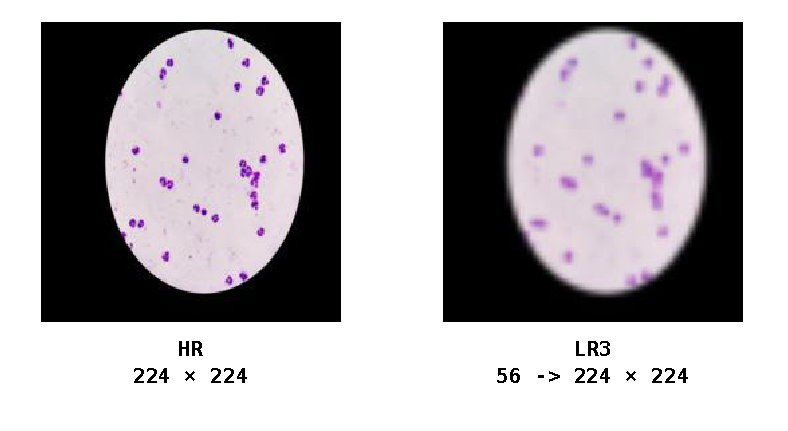
\includegraphics[width=0.68\textwidth]{figures/hr_lr3_comparison.pdf}
    }
    \caption{Example of the same thick blood smear image from patient folder \textbf{PvTk1} under the HR and LR3 resolution conditions.}
    \label{fig:resolution_comparison}
\end{figure}

\FloatBarrier

Keeping this preprocessing step simple was also important. As a result, the resolution reduction was implemented directly in the preprocessing pipeline.

\begin{lstlisting}[
    language=Python,
    caption={Resolution reduction used for the LR3 experiment.},
    label={lst:lr3_resize},
    xleftmargin=0.18\textwidth,
    xrightmargin=0.18\textwidth,
    frame=single
]
transforms.Resize((56, 56)),
transforms.Resize((224, 224)),
\end{lstlisting}

The same implementation is used for LR1 and LR2 by replacing the reduced resolution with \(160 \times 160\) pixels and \(112 \times 112\) pixels.

For validation and testing, no random augmentation is used. In the HR experiment, the images are only resized to \(224 \times 224\) pixels, converted to tensors, and normalised. In the case of a low-resolution experiment, the same resolution reduction used during training is also applied to the validation and test images before resizing them back to \(224 \times 224\) pixels. After that, the images are converted to tensors and normalised. This means that the same resolution condition is used for training, validation, and testing, while the random flips and rotations are only used during training to keep the results reliable.

For the external test with the Uganda dataset, the images were processed using the same LR3 test transform, first resized to \(56 \times 56\) pixels and then resized back to \(224 \times 224\) pixels. The already trained models were used directly without any retraining.

\section{Software Stack and Tools}

This work was developed in Python 3.12.2 and executed through the macOS Terminal. PyTorch was used as the main deep learning framework to build, train, and test the CNN models. Additionally, the torchvision library provided the pretrained network architectures (ResNet50, ResNet18 and MobileNetV3-Small) and also the image preprocessing transforms.

The microscope images were loaded by Pillow(PIL), while pandas read and handled the \textbf{labels.csv} file. The NumPy library managed the numerical operations, and to evaluate the developed models, scikit-learn was used to calculate metrics such as the confusion matrix, classification report, and ROC-AUC score. Matplotlib created the training curves, confusion matrices, and ROC curves.

When it comes to understanding how some models behave, the \textbf{pytorch-grad-cam} library plays a big role. It was used to generate Grad-CAM and Grad-CAM++ visualisations, which show which regions the model is concentrating on while making a prediction.

The scripts were also prepared to run directly from the Terminal. The Python \textbf{argparse} module is responsible for passing settings such as the dataset path, number of epochs, batch size, learning rate, and checkpoint folder as command-line arguments. The \texttt{--data-root} argument replaced the dataset path that was previously written directly in the script. This made the script more flexible, since it can be used with different dataset locations or on another computer without changing the path inside the Python file.

\begin{lstlisting}[
    language=Python,
    caption={Command-line arguments used in the training script.},
    label={lst:argparse},
    xleftmargin=0.10\textwidth,
    xrightmargin=0.10\textwidth,
    basicstyle=\ttfamily\small\color{blue},
    keywordstyle=\color{blue}\bfseries,
    commentstyle=\color{blue},
    stringstyle=\color{blue},
    identifierstyle=\color{blue}
]
def get_args():
    parser = argparse.ArgumentParser()
    parser.add_argument("--data-root", type=str, required=True)
    parser.add_argument("--labels-csv", type=str, default="labels.csv")
    parser.add_argument("--epochs", type=int, default=15)
    parser.add_argument("--batch-size", type=int, default=8)
    parser.add_argument("--lr", type=float, default=0.0001)
    parser.add_argument("--checkpoint-dir", type=str,
                        default="checkpoints")
    return parser.parse_args()
\end{lstlisting}

\begin{tcolorbox}[
    colback=gray!15,
    colframe=gray!50,
    boxrule=0.5pt
]

\textbf{Type and extent of AI use}

 \texttt{argparse} was first seen on some Kaggle competitions inside a python script. The idea sounded useful and Claude was then asked to create a similar function based on the
variables used in this work. Using the –data-root argument was also suggested by Claude instead of keeping the dataset path fixed inside the script.  Both were added to this project.

\vspace{0.4cm}

\textbf{The individual contribution}

The function was then integrated into the training script with the parameters that were used for the experiments, such as dataset path, epochs, batch size, learning rate, and checkpoint folder. 
The fixed dataset path was replaced with the \texttt{--data-root} argument.

\vspace{0.4cm}

\textbf{Critical evaluation of the AI contribution}

The \texttt{argparse} function is not necessary for the model, because the values could also be written directly in the script. But it made the work more flexible because the settings can be changed from the Terminal without going into the Python file every time. The \texttt{--data-root} argument was especially useful because the same script can now be used with a different dataset location without changing the source code.
\end{tcolorbox}

The training and testing scripts also include an automatic device selection. The scripts first check if a CUDA-supported GPU is available. If not, they check for the Apple MPS backend, and if neither is available, the CPU is used. Since the experiments in this work were executed on the MacBook Pro M2, the MPS backend was selected. The automatic device-selection logic was adapted from an example found on the PyTorch Forums.\footnote{\url{https://discuss.pytorch.org/t/same-model-gets-slightly-different-results-on-different-platforms/194551}, accessed 24 July 2026.}

\begin{lstlisting}[
    language=Python,
    caption={Automatic device selection adapted from a PyTorch Forum example.},
    label={lst:device_selection},
    xleftmargin=0.18\textwidth,
    xrightmargin=0.18\textwidth
]
if torch.cuda.is_available():
    device = torch.device("cuda")
elif torch.backends.mps.is_available():
    device = torch.device("mps")
else:
    device = torch.device("cpu")

print("using device:", device)
\end{lstlisting}

A GitHub repository was also created to make access to the model architectures and scripts easy for all team members, serving as a platform for version control, source code storage, and project updates.

The software versions used during the implementation are shown in Table~\ref{tab:software_versions}.

\begin{table}[htbp]
    \centering
    \caption{The software and library versions used in the implementation.}
    \label{tab:software_versions}
    \begin{tabular}{|l|l|}
        \hline
        \textbf{Software / Library} & \textbf{Version} \\ \hline
        Python & 3.12.2 \\ \hline
        PyTorch & 2.13.0 \\ \hline
        torchvision & 0.28.0 \\ \hline
        pandas & 2.2.2 \\ \hline
        NumPy & 1.26.4 \\ \hline
        Pillow & 10.4.0 \\ \hline
        scikit-learn & 1.5.1 \\ \hline
        Matplotlib & 3.10.0 \\ \hline
        pytorch-grad-cam & 1.5.5 \\ \hline
    \end{tabular}
\end{table}

\FloatBarrier

\section{Pipeline Architecture and Integration}
\label{sec:pipeline-architecture}


The implementation of the classification model is made of separate scripts, where each script is responsible for a specific stage of the overall pipeline. The pipeline consists of \textbf{build\_labels.py}, \textbf{dataset.py}, \textbf{train.py}, \textbf{test.py}, and \textbf{gradcam.py}. Keeping these scripts separated made it easier to reuse the same parts of the pipeline for different network architectures and also for reduced resolutions.

The pipeline starts with the NLM dataset folders, which offer a clean separation of the two classes (one folder for uninfected and 2 folders for infected: P. vivax and P. falciparum). The first script is \textbf{build\_labels.py} that goes through the three image folders and creates the \textbf{labels.csv} file. This CSV file stores the image path, class, binary label, patient ID, and the assigned dataset split. These generated information are then used by the \textbf{MalariaDataset} class in the second script which is \textbf{dataset.py}. This \textbf{MalariaDataset} class links the information from the CSV file to the actual image files and then loads the requested split (training, validation, or test).

The \textbf{dataset.py} script does not contain the preprocessing for the specific experiments. Instead, the preprocessing transforms are provided to the \textbf{MalariaDataset} class from the training or testing script. This means that the same dataset class can be reused for the HR, LR1, LR2, and LR3 experiments by only changing the corresponding transform pipeline.

During training, \textbf{train.py} loads the training and validation data through the defined \textbf{MalariaDataset} class. After that, the chosen CNN is configured for binary classification and trained with the given hyperparameters. After every epoch, the model is also evaluated on the validation set. After each validation step, the model is saved as \textbf{best\_model.pth} if its accuracy outperforms all previous epochs. This model represents the best model found during the training process.

After training, \textbf{test.py} loads the same CNN architecture used in training and the saved \textbf{best\_model.pth} checkpoint. The fixed test split is used for the final evaluation. During testing, the model parameters are not changed. The script calculates the evaluation metrics (accuracy, sensitivity, specificity, precision, f1-score and ROC-AUC) and also creates outputs such as the confusion matrix and ROC curve.

The main connection between the scripts and the generated files is shown in Figure~\ref{fig:implementation_pipeline}. The external test was not included in the figure because it uses a separate dataset and a separate testing script and does not form part of the main NLM training, validation, and testing pipeline.

\begin{figure}[htbp]
    \centering
    \fbox{
        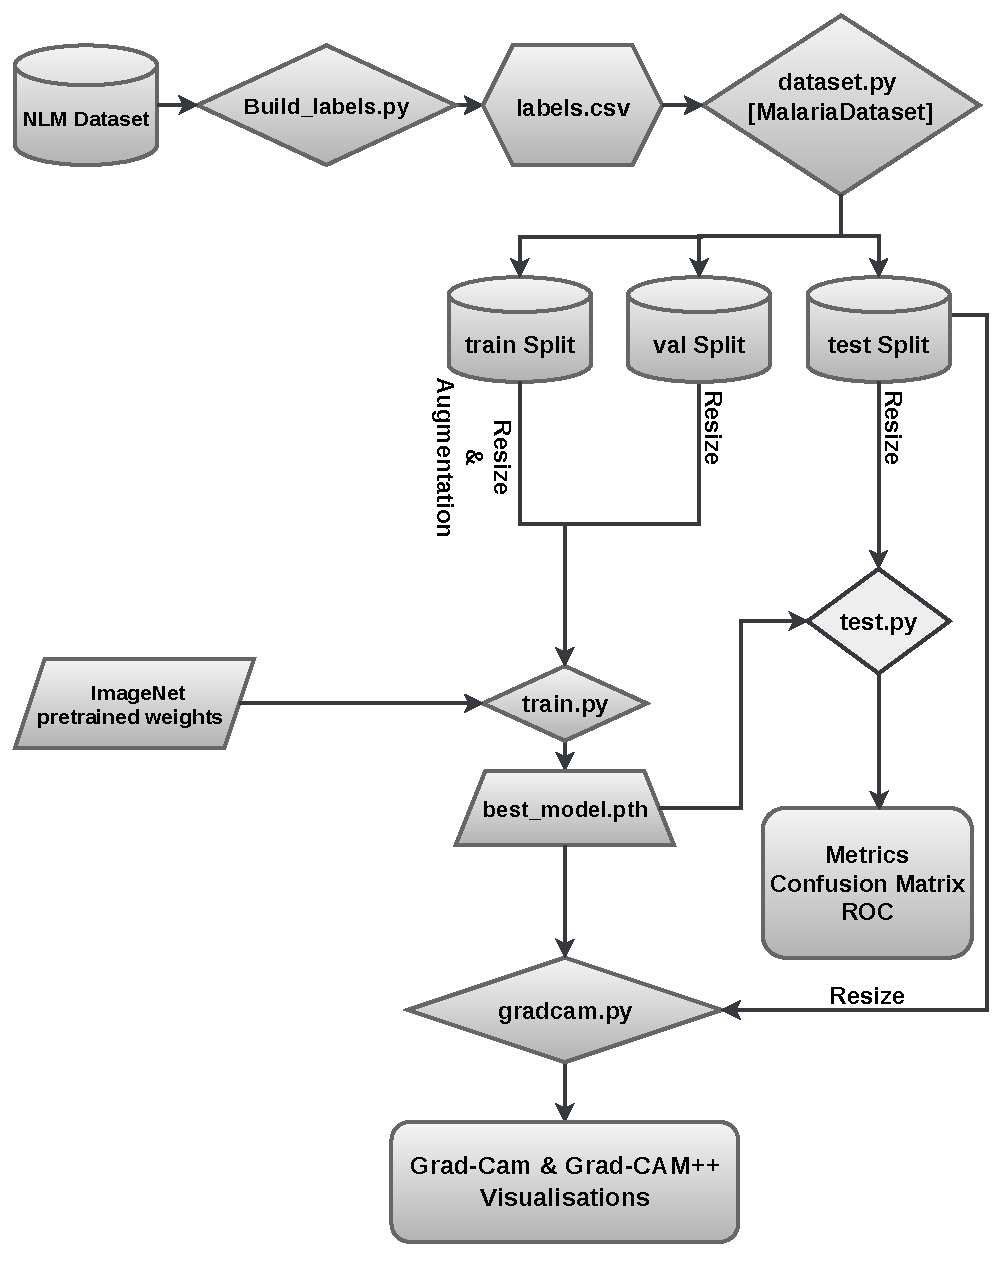
\includegraphics[width=0.85\textwidth]{figures/implementation_pipeline.pdf}
    }
    \caption{Script and data flow of the implemented classification pipeline.}
    \label{fig:implementation_pipeline}
\end{figure}

\FloatBarrier

For the external test, the same testing process was reused with a separate \textbf{labels\_uganda.csv} file and the script \textbf{test\_uganda.py}. The Uganda images were kept separate from the main NLM pipeline and were only used with already trained checkpoints, without any additional training or optimisation.

The last analysis step is conducted by \textbf{gradcam.py}. This script loads the already trained checkpoint from the training and uses images selected from the test set to generate Grad-CAM and Grad-CAM++ visualisations. In the \textbf{gradcam.py} script, the test predictions are first separated into true positive, true negative, false positive, and false negative groups. A limited number of examples from these groups are then used for the explainability analysis. The generated heatmaps are saved as image files for later visual evaluation and also for documentation purposes.

To keep the completed experiments separated from each other, each experiment was stored in its own folder together with the corresponding scripts and also the generated outputs. This made it easier to return to an older experiment without changing its original settings or results. It also helped when comparing the different architectures and resolution conditions. Furthermore, this separation allowed the team members to access the finished experiments without any complication.

The number of experiments was not the same for all three network architectures. ResNet50 was trained and tested at all four resolution conditions: HR, LR1, LR2, and LR3. ResNet18 and MobileNetV3-Small were trained and tested only at HR and LR3. This resulted in a total of eight main experiment runs. The different experiment runs are shown in Table~\ref{tab:experiment_coverage}.

\begin{table}[htbp]
    \centering
    \caption{Experiment runs for the three CNN architectures.}
    \label{tab:experiment_coverage}
    \begin{tabular}{|l|c|c|c|c|}
        \hline
        \textbf{Architecture} & \textbf{HR} & \textbf{LR1} & \textbf{LR2} & \textbf{LR3} \\ \hline
        ResNet50 & Yes & Yes & Yes & Yes \\ \hline
        ResNet18 & Yes & No & No & Yes \\ \hline
        MobileNetV3-Small & Yes & No & No & Yes \\ \hline
    \end{tabular}
\end{table}

\FloatBarrier

After completing the four resolution experiments with ResNet50, only two resolutions (HR and LR3) were selected for the comparison with ResNet18 and MobileNetV3-Small. These two conditions represent the two ends of the tested resolution range. HR represents the normal input condition, while LR3 with \(56 \times 56\) pixels represents the highest simulated resolution reduction used in this work. This made it possible to compare the three architectures under normal and strongly reduced image quality without repeating all four resolution experiments for every architecture.

The LR3 condition is relevant to the planned use of the model together with the smartphone-based ocular adapter. However, the \(56 \times 56\) pixel resolution is not a measured resolution of the final adapter. It was used only as a simulated worst-case resolution to investigate the behaviour of the models when the image detail is extremely reduced. 

Even though performance degraded across all architectures at LR3, the drop in specificity was the most obvious. Because MobileNet is lightweight and more suitable for future deployment, it was decided to optimise only this model. The original performance metrics for ResNet18 and ResNet50 were preserved as baseline comparisons.

The LR3 experiment on MobileNetV3-Small was then performed in three stages. The first stage used the same settings as the other architectures (ResNet50 and ResNet18): a learning rate of \(0.0001\), a batch size of 8, and 15 epochs. The training behaviour of this configuration was unstable.

For the first optimisation, the learning rate was reduced to \(0.00003\), the batch size was increased to 16, and the number of epochs was also increased to 30. These changes resulted in more stable training. After this optimisation, the classification was still not balanced enough between the two classes. That is why a second optimisation was performed by keeping the previous settings from the first optimisation and additionally adding class weights of \([2.0, 1.0]\) for the uninfected and infected classes. This made errors on the uninfected class have a higher influence on the training loss.

The three MobileNetV3-Small configurations are summarised in Table~\ref{tab:mobilenet_optimisation}.

\begin{table}[htbp]
    \centering
    \caption{MobileNetV3-Small configurations used for the LR3 experiment.}
    \label{tab:mobilenet_optimisation}
    \begin{tabular}{|l|c|c|c|c|}
        \hline
        \textbf{Configuration} & \textbf{Learning rate} & \textbf{Batch size} & \textbf{Epochs} & \textbf{Class weights} \\ \hline
        Baseline & 0.0001 & 8 & 15 & None \\ \hline
        Optimisation 1 & 0.00003 & 16 & 30 & None \\ \hline
        Optimisation 2 & 0.00003 & 16 & 30 & [2.0, 1.0] \\ \hline
    \end{tabular}
\end{table}

\FloatBarrier

This optimisation was deliberately limited to MobileNetV3-Small. As already discussed in Chapter~\ref{chap:concept-development}, the ResNet models are mainly used as stronger reference architectures for comparing classification performance, while MobileNet is more relevant for lightweight deployment. Re-optimising all three architectures was therefore outside the scope of this work. The numerical results of all experiments and the results of the MobileNet optimisations are presented later in Chapter~\ref{chap:testing}.

\section{Reproducibility}

The source code of the project is maintained in a GitHub repository and is available at \url{https://github.com/H-Yassine/malaria-diagnosis-master-thesis.git}.

The final version of the implementation used in this thesis corresponds to commit \textbf{\url{https://github.com/H-Yassine/malaria-diagnosis-master-thesis/commit/b256db2}}. The repository history contains \textbf{24 commits}, which document the development of the implementation between july 2026 and october 2026. In addition to the source code, the repository contains a \textbf{meetings/} folder where presentation files and project updates from the regular meetings were kept. The image datasets themselves are not distributed through the repository. The repository therefore provides only the code and pipeline structure, while the original datasets have to be obtained separately from their corresponding sources.

The structure of the repository is shown in Figure~\ref{fig:github_structure}. The project files are separated into four main folders: data, meeting documents, thesis files, and implementation scripts. Every experiment folder is stored inside the scripts folder of the repository.

\begin{figure}[htbp]
    \centering
    \fbox{
        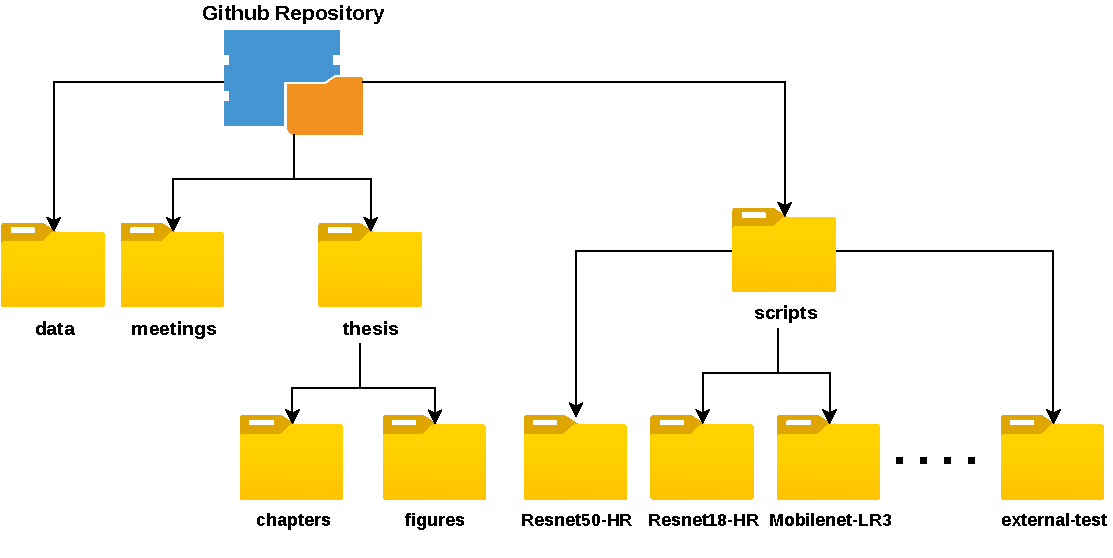
\includegraphics[width=0.88\textwidth]{figures/github-repo.pdf}
    }
    \caption{Overview of the GitHub repository structure.}
    \label{fig:github_structure}
\end{figure}

\FloatBarrier

The different experiments were organised in separate folders. Each of the eight main experiments contains the corresponding \textbf{dataset.py}, \textbf{train.py}, \textbf{test.py}, \textbf{labels.csv}, and the generated experiment outputs. Once an experiment was completed, its folder was kept unchanged so that later modifications did not affect already finished experiments. The Grad-CAM and Grad-CAM++ scripts were stored inside the corresponding experiment folders, while the external Uganda test was kept separately in its own \textbf{external-test/} folder.

Not all paths were handled in exactly the same way. For example, in \textbf{gradcam.py}, the dataset path and checkpoint path are defined at the beginning of the script, while other scripts use command-line arguments for some paths. This reflects the way the individual experiment scripts were developed and stored during the project.

An important part of the reproducibility is the fixed dataset split. The \textbf{build\_labels.py} script performs the 70/15/15 split at patient level and uses a fixed random seed of 42. This means that running the script again with the same dataset produces the same patient assignment for training, validation, and testing. The resulting assignments are stored in \textbf{labels.csv} and reused throughout the experiments. Each experiment also keeps its \textbf{best\_model.pth} checkpoint together with its result files and visual outputs. Information about the datasets is additionally documented in a \textbf{README.md} file inside the \textbf{data/} folder. 

There are still some limits to reproducibility. The fixed seed of 42 controls the patient split, but the training scripts do not fix all random operations with a global PyTorch seed. Random data augmentation and model training can therefore produce small differences when an experiment is trained again. The experiments were also executed using the Apple MPS backend, where exact numerical results are not guaranteed to be identical between repeated runs. For this reason, the saved checkpoints and result files are kept together with each completed experiment. In addition, the external image datasets cannot be redistributed with the source code and have to be downloaded separately from their original providers.



















